\documentclass[discrete.tex]{subfiles}

\begin{document}
\section{Задача о максимальном паросочетании в графе. Алгоритм построения}

\begin{definition}
    Граф $<M, N>$ называется простым или двудольным, если множество его вершин разбито на два
    множества $M_b$ и $M_c$ и все начала дуг принадлежат $M_b$, а концы $M_c$
\end{definition}

\begin{definition}
    Набор ребер $J \subset N$ называется паросочетанием, если $\forall j_1, j_2 \in J,\ \
    j_1 \neq j_2$ начала и концы этих дуг различны
\end{definition}

\begin{definition}
    Максимальное паросочетание - максимальное по числу ребер паросочетание
\end{definition}

\begin{definition}
    Цепью длины $k$ называется некоторый простой путь, содержащий $k$ ребер
\end{definition}

\begin{definition}
    Чередующей цепью (относительно некоторого паросочетания) называется цепь,
    в которой ребра поочередно принадлежат/не принадлежат паросочетанию.
\end{definition}

\begin{definition}
    Увеличивающей цепью называется чередующаяся цепь, у которой начальная и конечная
    вершины не принадлежат паросочетанию
\end{definition}

\begin{theorem}[Бержа]
    Паросочетание является максимальным $\rla$ $\cancel{\exists }$ увеличивающих
    относительно него цепей
\end{theorem}

\begin{definition}
    Насыщенная вершина - принадлежащая паросочетанию
\end{definition}

\begin{definition}[Алгоритм Куна]
    Из каждой ненасыщенной вершины графа (из одной доли) будем искать увеличивающую цепь.
    Для это применим DFS (поиск в глубину). Мы выбрали ненасыщенную вершину $v$, рассмотрим все вершины,
    инцидентные с ней. Назовем текущую вершину $to$, если она ненасыщенная, то мы
    нашли увеличивающую цепь, иначе запустим поиск от вершины $p$ ($(v, to), \ (to, p)$)
    пробуем найти увеличивающую цепь из нее.\\
    Если из вершины $p$ мы нашли увеличивающую цепь, то "прочередуем"\ ребра. Уберем
    ребро $(p, to)$ и добавим $(v, to)$\\
    После того, как все вершины будут просмотрены, текущее паросочетание будет
    максимальным.
\end{definition}

\begin{figure}[H]
        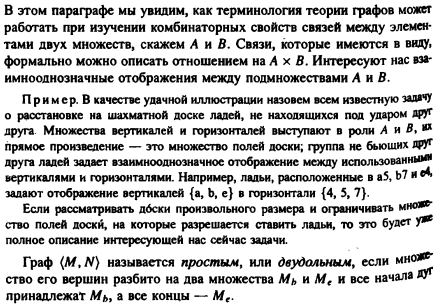
\includegraphics[width=10cm]{pics/49_1}
        \centering
\end{figure}

\begin{figure}[H]
        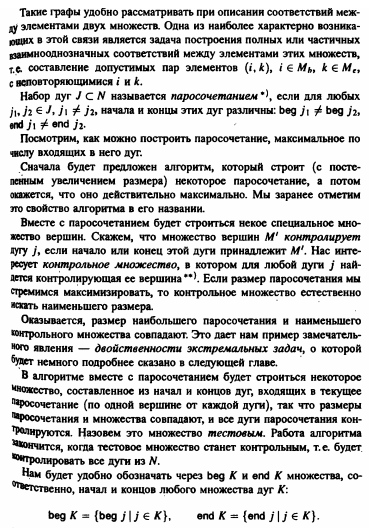
\includegraphics[width=10cm]{pics/49_2}
        \centering
\end{figure}

\begin{figure}[H]
        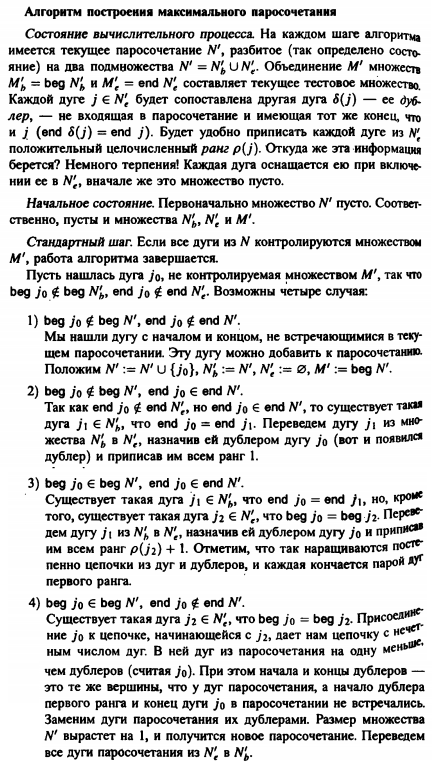
\includegraphics[width=10cm]{pics/49_3}
        \centering
\end{figure}

\begin{figure}[H]
        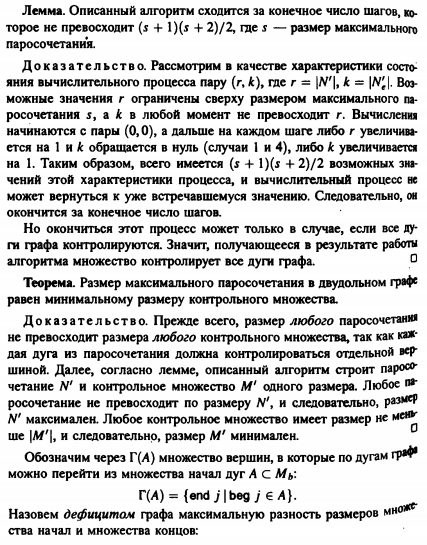
\includegraphics[width=10cm]{pics/49_4}
        \centering
\end{figure}

\begin{figure}[H]
        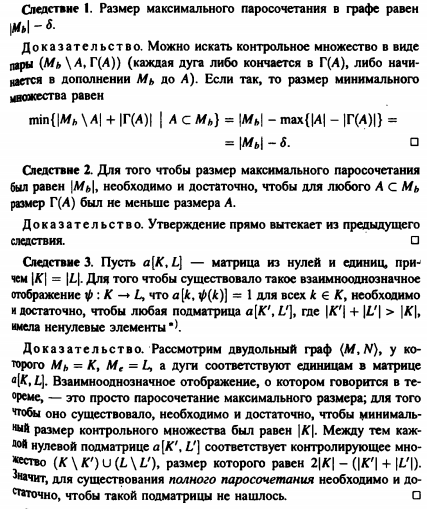
\includegraphics[width=10cm]{pics/49_5}
        \centering
\end{figure}

\begin{figure}[H]
        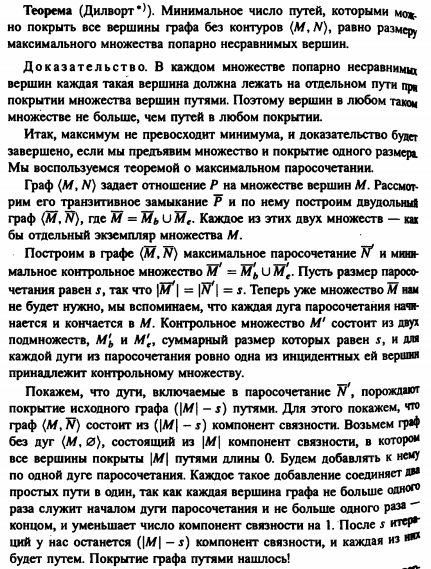
\includegraphics[width=10cm]{pics/49_6}
        \centering
\end{figure}

\begin{figure}[H]
        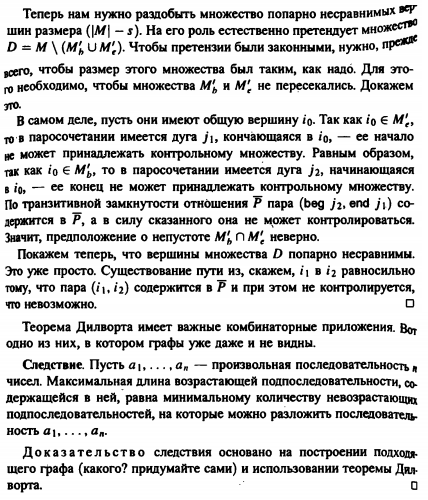
\includegraphics[width=10cm]{pics/49_7}
        \centering
\end{figure}

\begin{figure}[H]
        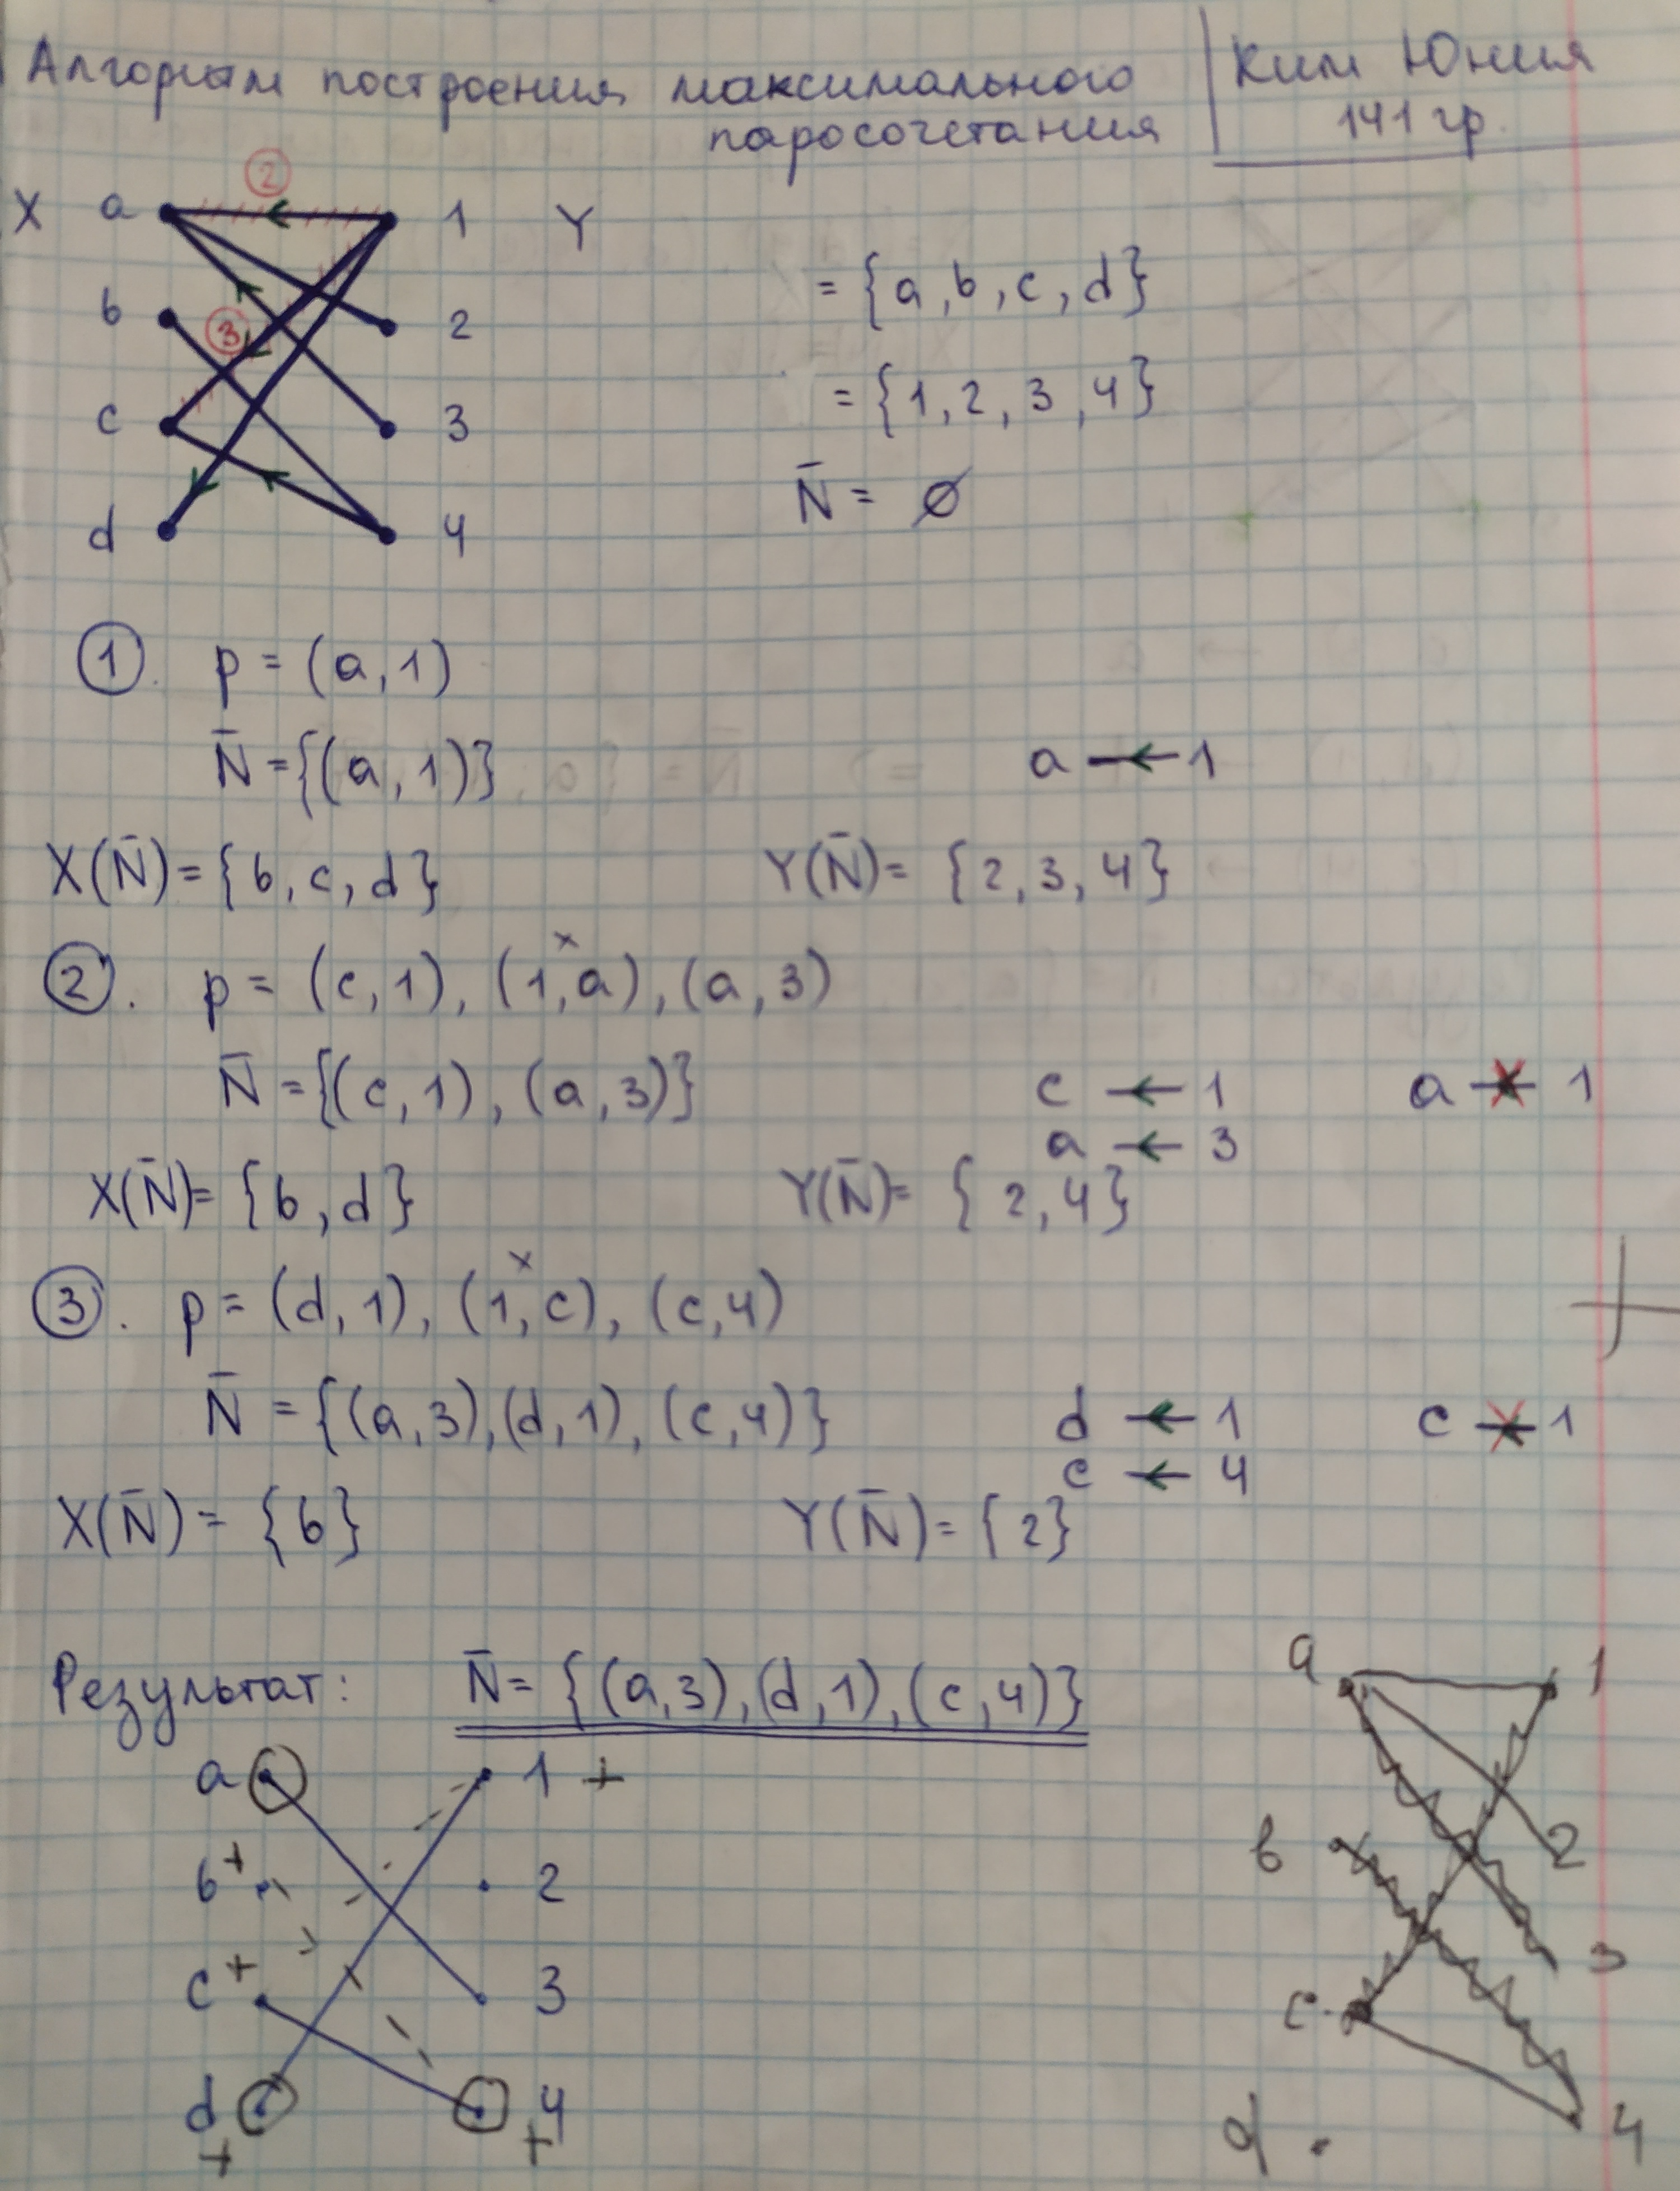
\includegraphics[width=10cm]{pics/49_8}
        \centering
\end{figure}

\end{document}
